% The format of this file must be strictly retained to avoid problems
% in the generation of examples.html
\bfig{
    \centerline{\getpic{quick}}
    \caption{The quick-start example from the manual
    \src{quick.m4}.}
  }

\bfig{
    \centerline{{\small\getpic{CctTable}}}
    \caption{Two-terminal elements, showing some variations
    \src{CctTable.m4}.}
  }

\bfig{
    \centerline{\getpic{Diodes}}
    \caption{Diodes
    \src{Diodes.m4}.}
  }

\bfig{
    \centerline{\getpic{Emarrows}}
    \caption{Radiation arrows
    \src{Emarrows.m4}.}
  }

\bfig{
    \centerline{\getpic{Sources}}
    \caption{Sources and source-like elements
    \src{Sources.m4}.}
  }

\bfig{
    \centerline{\getpic{Variable}}
    \caption{Arrows and marks indicating variability
    \src{Variable.m4}.}
  }

\bfig{
    \centerline{\getpic{AmpTable}}
    \caption{Macros {\tt amp}, {\tt delay}, and {\tt integrator}
    \src{AmpTable.m4}.}
  }

\bfig{
    \centerline{\getpic{Switches}}
    \caption{The {\tt switch} and {\tt dswitch} macros
    \src{Switches.m4}.}
  }

\bfig{
    \centerline{\getpic{Fuses}}
    \caption{Macros {\tt fuse} and {\tt cbreaker}
    \src{Fuses.m4}.}
  }

\bfig{
    \centerline{\getpic{Grounds}}
    \caption{Ground symbols
    \src{Grounds.m4}.}
  }

\bfig{
    \centerline{\getpic{Antennas}}
    \caption{Antenna symbols
    \src{Antennas.m4}.}
  }

\bfig{
    \centerline{\getpic{Audio}}
    \caption{Audio elements
    \src{Audio.m4}.}
  }

\bfig{
    {\small\centerline{\getpic{Opamp}} }
    \caption{The opamp
    \src{Opamp.m4}.}
  }

\bfig{
    {\small\centerline{\getpic{Xform}} }
    \caption{The transformer element, drawing direction down
    \src{Xform.m4}.}
  }

\bfig{
    \centerline{\getpic{Relay}}
    \caption{The {\tt contact} and {\tt relay} macros
    \src{Relay.m4}.}
  }

\bfig{
    \centerline{\getpic{ujt}}
    \caption{UJT examples
    \src{ujt.m4}.}
  }

\bfig{
    \centerline{\getpic{fet}}
    \caption{FETs, showing programmable components and example customizations
    \src{fet.m4}.}
  }

\bfig{
    \centerline{\getpic{thyristor}}
    \caption{Thyristor examples
    \src{thyristor.m4}.}
  }

\bfig{
    \centerline{\getpic{Bip}}
    \caption{Bipolar transistors (drawing direction: up)
    \src{Bip.m4}.}
  }

\bfig{
    \centerline{\getpic{Tgate}}
    \caption{The {\tt tgate} and {\tt ptrans} elements
    \src{Tgate.m4}.}
  }

\bfig{
    \centerline{\getpic{Nport}}
    \caption{The {\tt nport} and {\tt nterm} macros
    \src{Nport.m4}.}
  }

\bfig{
    \centerline{\getpic{NLG}}
    \caption{Some customizations of {\tt nport}
    \src{NLG.m4}.}
  }

\bfig{
    \centerline{\getpic{Windings}}
    \caption{The macro {\tt winding(L|R,diam,pitch,turns,core wid,core color)}
    \src{Windings.m4}.}
  }

\bfig{
    \centerline{\getpic{ex01}\quad
                \getpic{Timer}}
    \caption{Two simple labeled circuits
    \src{ex01.m4}%
    \src{Timer.m4}.}
  }

\bfig{
    \centerline{\getpic{Sixpole}}
    \caption{A six-pole filter
    \src{Sixpole.m4}.}
  }

\bfig{
    \centerline{\getpic{MC}}
    \caption{A three-phase switched AC-AC converter
    \src{MC.m4}.}
  }

\bfig{
    \centerline{\getpic{ex18}\hspace*{10ex}
      \raisebox{\baselineskip}{\getpic{ex19}}}
    \caption{Precision half-wave rectifier and a tunnel diode circuit
      (illustrating {\tt opamp, diode, resistor, ground,} and labels)
    \src{ex18.m4}%
    \src{ex19.m4}.}
  }

\bfig{
    \centerline{\getpic{ex10}\hspace*{10ex}
      \getpic{bistable}}
    \caption{Non-planar graph and bistable circuit
     (illustrating the {\tt crossover} macro and colored elements)
    \src{ex10.m4}%
    \src{bistable.m4}.}
  }

\bfig{
    \centerline{\getpic{Three}}
    \caption{Three-phase oscillator
    \src{Three.m4}.}
  }

\bfig{
    \centerline{\raisebox{0.5in}{\getpic{gpar}}\hspace*{10ex}
      \getpic{ex17}}
    \caption{A skewed circuit used to test the macro
      {\tt gpar\_(}{\sl element}, {\sl element}, {\sl separation}{\tt )},
      and a repetitive network created by Pic looping
    \src{gpar.m4}%
    \src{ex17.m4}.}
  }

\bfig{
    \centerline{\getpic{ex12}}
    \caption{ A CMOS NAND gate, a test circuit, and an XMOSFET example
    \src{ex12.m4}.}
  }

\bfig{
    \centerline{\getpic{pwrsupply}}
    \caption{An elementary power supply circuit with colored elements,
      and a multiple-winding transformer with 3-phase rectifier
    \src{pwrsupply.m4}.}
  }

\bfig{
    \centerline{\getpic{TTLnand}}
    \caption{ TTL NAND gate illustrating a transistor with multiple emitters
    \src{TTLnand.m4}.}
  }

\bfig{
    \centerline{\getpic{I2L}}
    \caption{ Gate circuit and equivalent embedded $I^2L$ components
      illustrating multiple collectors
    \src{I2L.m4}.}
  }

\bfig{
    \centerline{\getpic{ex11}}
    \caption{Transistor radio audio chain (a modest circuit with a few
      custom elements)
    \src{ex11.m4}.}
  }

\bfig{
    \centerline{\getpic{Csource}}
    \caption{Realization of a controlled source
        (illustrating stacked element labels)
    \src{Csource.m4}.}
  }

\bfig{
    \centerline{\getpic{Drive}}
    \caption{Synchronous machine driven by variable-speed drive and rectifier
    \src{Drive.m4}.}
  }

\bfig{
    \centerline{\getpic{ex04}}
    \caption{Labels on non-manhattan elements
    \src{ex04.m4}.}
  }

\bfig{
    \centerline{\getpic{ex16}}
    \caption{A rate $1/2$ binary convolutional coder and its state diagram
    \src{ex16.m4}.}
  }

\bfig{
    \centerline{\getpic{ex03}}
    \caption{Digital filter
    \src{ex03.m4}.}
  }

\begin{sidewaysfigure} %\rotatebox{90}{% \begin{landscape} %ignore%
\bfig{
    \centerline{\hspace*{2cm}\getpic{lcct}}
    \caption{A digital circuit of moderate size,
      redrawn from M.~P.~Maclenan and G.~M.~Burns,
      ``An Approach to Drawing Circuit Diagrams for Text Books,''
      Tugboat (12)1, March 1991, pp.\ 66-69
    \src{lcct.m4}.}
  }
\end{sidewaysfigure} %}% \end{landscape}

\bfig{
    \centerline{\getpic{ex02}}
    \caption{Elements at obtuse angles
    \src{ex02.m4}.}
  }

\bfig{
    \centerline{\getpic{sfg}}
    \caption{Signal-flow graphs
    \src{sfg.m4}.}
  }

\bfig{
    \centerline{\getpic{Logic}}
    \caption{Basic logic gates
    \src{Logic.m4}.}
  }

\bfig{
    \centerline{\getpic{ex08}}
    \caption{General-purpose latch: a small logic circuit
    \src{ex08.m4}.}
  }

\bfig{
    \centerline{\getpic{Decoder}}
    \caption{Decoder logic, constructed using the {\tt for\_} macro
    \src{Decoder.m4}.}
  }

\bfig{
    \centerline{\getpic{ex21}}
    \caption{Some flip-flops
    \src{ex21.m4}.}
  }

\bfig{
    \centerline{\getpic{ShiftR}}
    \caption{A 5-bit shift register drawn using a custom flip-flop
    \src{ShiftR.m4}.}
  }

\bfig{
    \centerline{\getpic{CanLogic}}
    \caption{A way of automatically drawing two-layer logic diagrams
    \src{CanLogic.m4}.}
  }

\bfig{
    \centerline{\getpic{control}}
    \caption{Control-system block diagrams that do not require m4
    \src{control.m4}.}
  }

\bfig{
    \centerline{\getpic{ex00}\quad\quad
      \getpic{ex07}}
    \caption{Line diagrams
    \src{ex00.m4}%
    \src{ex07.m4}.}
  }

\bfig{
    \centerline{\getpic{exp}\quad
                \getpic{Globe}}
    \caption{Test of {\tt project} and other {\tt lib3D}
      macros, showing the projection of a solid onto
      the $y_1,z_1$ plane by sighting along the $x_1$ axis.
    \src{exp.m4}%
    \src{Globe.m4}.}
  }

\bfig{
    \centerline{\getpic{graysurf}}
    \caption{Plotting a surface using a gray scale
    \src{graysurf.m4}.}
  }

\bfig{
    \centerline{\getpic{ex09}}
    \caption{Illustrating the macro
      {\tt dimension\_(}{\sl linespec}, {\sl offset}, {\sl label},
      {\tt D|H|W|}{\sl blank width}, {\sl tic offset},{\tt <-|->)}.
      A negative second argument implies an offset to the right of the
      {\sl linespec} direction.  A {\sl label} starting with {\tt "} or
      {\tt sprintf} is copied literally.  If {\sl label} is an
      {\tt s\_box(...)} then setting argument 4 to {\tt H}, {\tt W}, or
      {\tt D} tailors the blank width to the {\tt s\_box} height, width, or
      diagonal respectively; i.e.,\ {\tt W} is equivalent to
      {\tt s\_wd+textoffset*2}
    \src{ex09.m4}.}
  }

\bfig{
    \centerline{\getpic{ex05}}
    \caption{Use of {\tt darrow}
    \src{ex05.m4}.}
  }

\bfig{
    \centerline{\getpic{ex06}}
    \caption{Crosshatching by {\tt for} loops
    \src{ex06.m4}.}
  }

\bfig{
    \centerline{\getpic{Loglog}}
    \caption{A graph drawn using the pic language 
    \src{Loglog.m4}.}
  }

\bfig{
    \centerline{\getpic{csc}}
    \caption{Conestoga Sailing Club (illustrating the filling of arbitrary
      shapes)
    \src{csc.m4}.}
  }

\bfig{
    \centerline{\getpic{rose}}
    \caption{Redrawn from a detail of the set design for the musical
      {\it Dracula,} used for testing {\tt dpic}.  This diagram
      consumes much \LaTeX\ main memory  but can be produced as the raw
      postscript output of {\tt dpic -r} since no text formatting is
      required
    \src{rose.m4}.}
  }

\bfig{
    \centerline{\getpic{diamond}}
    \caption{Variations on M.~Goossens, S.~Rahtz, and F.~Mittelbach,
      {\em The \LaTeX\ Graphics Companion,} Addison-Wesley 1997, pp.\ 57-58
    \src{diamond.m4}.}
  }

\bfig{
    \centerline{\getpic{worm}}
    \caption{An exercise in calculating RGB colours
    \src{worm.m4}.}
  }

\bfig{
    \centerline{\getpic{Sierpinski}}
    \caption{The Sierpinski triangle: a test of pic macro recursion
    \src{Sierpinski.m4}.}
  }

\bfig{
    \centerline{\getpic{recycle}\hspace*{10ex}
      \getpic{yinyang}}
    \caption{Modest repetition and partial fill
    \src{recycle.m4}%
    \src{yinyang.m4}.}
  }

\bfig{
    \centerline{\getpic{ex15}}
    \caption{Simple diagrams that are easily drawn by looping
    \src{ex15.m4}.}
   }

\bfig{
    \centerline{\getpic{Btree}}
    \caption{A binary tree
    \src{Btree.m4}.}
  }

\bfig{
    \centerline{\getpic{Flow}}
    \caption{A flowchart sampler
    \src{Flow.m4}.}
  }

% Overlaying a figure with line graphics depends on the postprocessor format:
\ifpst%                          PSTricks
\bfig{%
    \centerline{\getpic{Incleps}}%
    \caption{Overlaying a figure with line graphics
    \src{Incleps.m4}.}%
  }
\else\ifpgf%                     PGF
\bfig{%
    \centerline{\getpic{Incleps}}% %ignore%
    \caption{Overlaying a figure with line graphics %ignore%
    \src{Incleps.m4}.}%
  }
\else\ifmpost%                   MetaPost
\bfig{%
    \centerline{\boxdims{InclA}{%ignore%
        \includegraphics[width=3in]{../Incl.eps.gz}}%
        \hspace*{-3in}\includegraphics{Inclpdf.1}}%
    \caption{Overlaying a figure with line graphics %ignore%
    \src{Inclpdf.m4}.}
  }
\else\ifpdfl%                    pdflatex
\bfig{%
    \centerline{\boxdims{InclA}{%ignore%
        \includegraphics[width=3in]{../Incl}}%
        \hspace*{-3in}\includegraphics{Inclpdf}}%
    \caption{Overlaying a figure with line graphics %ignore%
    \src{Inclpdf.m4}.}
  }
\else\ifpostscript%              Postscript with psfrag (.eps.gz not allowed)
\bfig{%
    \centerline{\boxdims{InclA}{%ignore%
        \includegraphics[width=3in]{Incl.eps}}%
        \hspace*{-3in}\includegraphics{Inclpdf.eps}}%
    \caption{Overlaying a figure with line graphics %ignore%
    \src{Inclpdf.m4}.}
  }
\fi\fi\fi\fi\fi

\end{document}
